\documentclass{ieeetj}
\newcommand{\seclogo}{}
\usepackage{cite}
\usepackage{amsmath,amssymb,amsfonts}
\usepackage{listings}
\usepackage{algorithmic}
\usepackage{graphicx,color}
\usepackage{textcomp}
\usepackage{hyperref}
\usepackage{float}
\usepackage[table,xcdraw]{xcolor}
\definecolor{blau}{RGB}{198, 220, 255} 
\definecolor{gris}{RGB}{176, 176, 176}
\definecolor{verd}{RGB}{ 173, 240, 199}

\hypersetup{hidelinks=true}
\usepackage{algorithm,algorithmic}
\lstset{
    language=Java,
    basicstyle=\ttfamily\small,
    keywordstyle=\bfseries\color{blue},
    stringstyle=\color{red},
    morecomment=[l][\color{magenta}]{//},
    frame=single,
    breaklines=true,
    showstringspaces=false,
    tabsize=1,
}
\def\BibTeX{{\rm B\kern-.05em{\sc i\kern-.025em b}\kern-.08em
    T\kern-.1667em\lower.7ex\hbox{E}\kern-.125emX}}
\AtBeginDocument{\definecolor{tmlcncolor}{cmyk}{0.93,0.59,0.15,0.02}\definecolor{NavyBlue}{RGB}{0,86,125}}

% Definim el logo
\def\OJlogo{
    \vspace{-14pt} % Espai negatiu per pujar el logo
    
\includegraphics[height=0.96cm]{png/logo.png}}

\begin{document}
\receiveddate{19 Juny, 2025}
\publisheddate{22 Juny, 2025}
\currentdate{21 Juny, 2025}

\title{Programació criptogràfica: \newline Encriptació amb RSA}

\author{Daniel García} \affil{Universitat de les Illes Balears, Departament d'Enginyeria Informàtica} \corresp{Autor de contacte: Daniel García (email: daniel.garcia19@estudiant.uib.es)}



\begin{abstract}

En aquest document es presenta el desenvolupament d'una aplicació implementada en Java que permet l'encriptació i desencriptació d'arxius. L'objectiu principal és determinar la viabilitat d'aquesta tècnica

L'algorisme criptogràfic emprat es el RSA, de tipus de clau pública, que està basat en la factorització de nombres primers molt grans.

Com a funcionalitats addicionals, s'ha implementat la possibilitat de comprimir amb Huffman els arxius encriptats, a més d'una gestió persistent de les claus, ús de concurrència i reportatge del temps emprat. 

\end{abstract}

\begin{IEEEkeywords}
RSA, nombres primers, Criptografia, Swing, MVC, Huffman, Clau pública, Clau privada, Ciberseguretat, Java 
\end{IEEEkeywords}


\maketitle
\section{Introducció}
La criptografia és una branca molt important de la informàtica, sobretot en un mon hiperconnectat on la privadesa i la seguretat estan en primera plana.  \newline
En el marc de l’assignatura d’Algorismes Avançats, aquesta pràctica se centra en aplicar la teoria donada sobre el xifrat RSA a una pràctica on es pugui demostrar els coneixements adquirits al llarg del curs.\newline

Aquest projecte explora l’ús d’algorismes probabilístics basats en mostreig Monte Carlo\cite{hammersley1964} per calcular ràpidament nombres primers. \newline
A més, s’implementa l'algorisme RSA per obtenir una encriptació de clau pública .\newline

La solució es construeix segons el patró Model–Vista–Controlador (MVC) \cite{gamma1994}, garantint la separació de responsabilitats entre la capa de dades i lògica (Model), la interfície d’usuari (Vista) i el control del flux (Controlador). \newline
Finalment, la GUI es desenvolupa íntegrament amb Java Swing \cite{gafter1999}, complint els requisits d’interacció i visualització sense utilitzar la consola en cap moment.

\section{Marc Teòric}
\subsection{RSA}
RSA es sistema criptogràfic\cite{RSA} àmpliament utilitzat en l'àmbit de la criptografia, tant per xifrar arxius con per signar-los. RSA es un sistema de clau publica i privada \cite{pubkey}, que permet la transmissió segura d'informació per la xarxa, entre d'altres. El xifrat es basa en la complexitat computacional que suposa factoritzar un nombre semiprimer, un nombre que només es pot formar per la multiplicació de dos nombres primers.

\subsection{Mostreig Monte Carlo}
El mostreig Monte Carlo és una tècnica per estimar propietats d’una població a partir de mostres aleatòries \cite{hammersley1964}. Aplicat a nombres primers, el test de primalitat de Miller-Rabin \cite{miller} permet trobar nombres primers de gran mida amb una alta probabilitat d'encert. Això es possible al triar testimonis de forma aleatòria en un temps de \(O(log^3n*log(1/\epsilon))\) sent \(\epsilon\) l'error causat. Aquest test es àmpliament usat en aplicacions on es depèn de nombres primers.



\subsection{Codificació de Huffman}
La codificació de Huffman \cite{huffman1952} es altament emprada per comprimir sense pèrdua arxius de forma eficaç.
L'algorisme consisteix en crear una taula de freqüències per després generar un arbre binari per assignar un codi a cada símbol.




\section{Entorn de Programació}
Per al desenvolupament d’aquesta pràctica s’ha configurat un entorn de treball basat en les eines i tecnologies següents:

\begin{itemize}
  \item \textbf{Llenguatge de programació:} Java SE 23. S’ha triat per la seva robustesa, portabilitat i per disposar de llibreries estàndard per a la gestió de fils a alt nivell \texttt{ExecutorService}.
  \item \textbf{Interfície gràfica:} Java AWT i Swing. Swing s’empra per construir la GUI complint el patró MVC\cite{gamma1994} i permet gestionar esdeveniments i components gràfics de manera eficient\cite{gafter1999}.
  \item \textbf{IDE:} IntelliJ IDEA. Aquest entorn integrat facilita la navegació pel codi, la refactorització automàtica, la detecció d’errors en temps real i la integració amb sistemes de compilació com Maven o Gradle.
  \item \textbf{Control de versions:} Git amb repositori a GitHub. Permet portar un historial complet de canvis, gestionar branques de desenvolupament i col·laborar de forma distribuïda.
  \item \textbf{Documentació científica:} LaTeX a Overleaf mitjançant la plantilla IEEEtran. Facilita la redacció col·laborativa, la gestió de citacions i el format segons l’estàndard IEEE.
\end{itemize}

\noindent
L’estructura del projecte segueix el patró Model–Vista–Controlador:
\begin{description}
  \item\textbf{Model:} Classes \texttt{Dades} i les diferents classes com \texttt{EncriptadorDesencriptador}, responsables de l’emmagatzematge de les claus, generar les claus RSA i l'encriptació i desencriptació.
  
  \item\textbf{Vista:} Classe \texttt{Finestra} (extensió de \texttt{JFrame}), amb tots els components Swing (botons, etiquetes, \texttt{JFileChooser}, etc.).
  \item\textbf{Controlador:} Classe \texttt{Main} (implementa la interfície \texttt{Comunicar}), que enllaça la vista i el model, registra listeners d’esdeveniments i invoca les operacions de xifrat, gestió i compressió.
\end{description}




\section{Desenvolupament i Metodologia}

\subsection{Arquitectura general del sistema}
El projecte s'ha estructurat seguint el patró \textbf{Model–Vista–Controlador (MVC)}, que permet una clara separació de responsabilitats:
\begin{itemize}
    \item \textbf{Model}: La interfície \texttt{Comunicar.Java} juntament amb la classe principal del programa \texttt{Main.java} són els responsables d'establir la comunicació i alinear les parts del programa per poder comunicar les peticions de l'usuari, executar l'algorisme classificador corresponent i mostrar els resultats obtinguts.
    
    \item \textbf{Vista}: Implementada amb Swing, proporciona una interfície gràfica intuïtiva i flexible per a la interacció amb l'usuari. Mostra els resultats del xifrat com les claus disponibles. 

\item \textbf{Controlador}: Actua com a intermediari, processant els esdeveniments de la GUI i invocant accions sobre el \textbf{Model}, a través de la interfície \textit{Comunicar} i la classe \textit{Main.java}.

\end{itemize}
\subsection{Estructura de paquets i classes}
L'estructura del programa segueix les bones pràctiques d'encapsulament de Java. 
Els paquets principals es poden identificar d'acord amb el disseny de l'arquitectura Model-Vista-Controlador. 
La figura següent il·lustra l'estructura del nostre programa. \newline
Els quadres de colors representen diferents elements: \textcolor{blau}{els blaus}, les \textbf{classes}; \textcolor{gris}{els grisos}, les \textbf{interfícies};\textcolor{verd}{ i els altres}, els \textbf{paquets}. CAMBIAR

\begin{figure}[H]
    \centering
    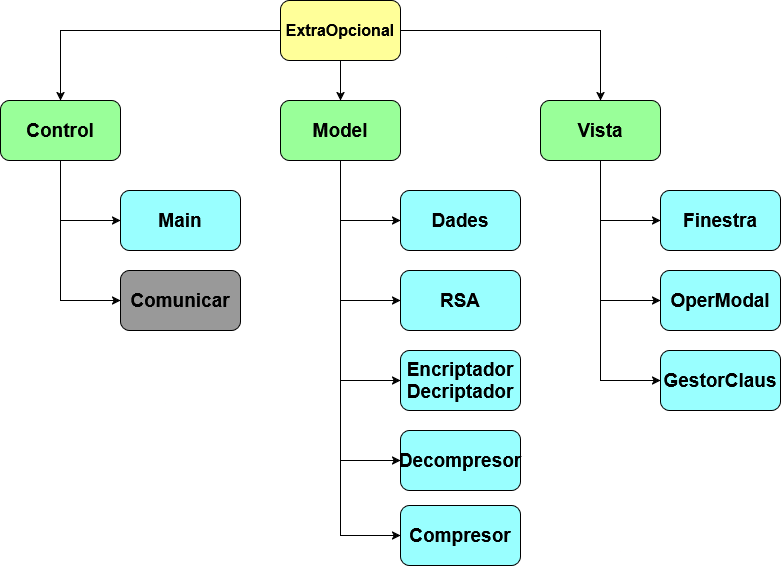
\includegraphics[width=0.5\linewidth]{png/praExtra.png}
    \caption{Classes principals del projecte}
    \label{fig:enter-label}
\end{figure}
\subsection{Implementació del xifrat RSA}
El xifrat RSA està implementat a la classe \texttt{RSA.java}, que realitza els passos següents:
\begin{enumerate}
  \item Obtenció amb algorismes probabilístics dels nombres primers $P$ i $Q$.
  \item Càlcul de $N = PQ$.
  \item Càlcul de $\phi(N) = (P-1)(Q-1)$.
  \item Càlcul de $E$ tal que $1 < E < \phi(N)$ i $E$ i $\phi(N)$ son coprimers.
  \item Càlcul de $D$ tal que $(DE\mod \phi(N)=1$
  \item Crear les claus públiques i privades:
    \begin{itemize}
      \item Clau pública (encriptar) $(E, N)$
      \item Clau privada (desencriptar) $(D, N)$
    \end{itemize}
  \item Per operar amb una clau es calcula $res = val^{E|D}\mod N$
\end{enumerate}

\begin{lstlisting}[language = Java, breaklines = true]
// Excerpt de RSA.generar()
for (int i = 0; i < 3; i++) {
    calls.add(executor.submit(() -> prim.otroProbablePrimo(new BigInteger("1" + "0".repeat(n)))));
}
P = calls.get(0).get();
Q = calls.get(1).get();
E = calls.get(2).get();

calls.add(executor.submit(() -> P.multiply(Q)));
calls.add(executor.submit(() -> P.add(new BigInteger("-1")).multiply(Q.add(new BigInteger("-1")))));
N = calls.get(3).get();
FN = calls.get(4).get();

if (E.compareTo(FN) > -1){
    throw new RuntimeException("E is greater than FN");
}

D = E.modInverse(FN);
 
\end{lstlisting}

\subsection{Xifrat i desxifrat d'informació}
Per xifrar un arxiu, o desxifrar, primer es divideix en tantes parts com nuclis té el processador, a continuació cada part s'opera respectivament de forma concurrent i finalment es forma el fitxer final.
\begin{lstlisting}
byte[] fileIn = bis.readAllBytes();

int _step = fileIn.length / N_THREADS;
final int step = _step + 1 - (_step % N_THREADS);
for (int i = 0; i < N_THREADS -1; i++) {
    final int j = i;
    byte[] finalFileIn = fileIn;
    addConcurrent(() -> {
        encriptar(finalFileIn, j, j * step, (j+1) * step);
    });
}
byte[] finalFileIn1 = fileIn;
addConcurrent(() -> {
    encriptar(finalFileIn1, N_THREADS-1, (N_THREADS-1) * step, finalFileIn1.length);
});

waitAll();

try(BufferedOutputStream bos = new BufferedOutputStream(new FileOutputStream(outPath))){
    byte[] header = CryptHeader.createHeader(rsa, comprimir);
    bos.write(header);
    for (ArrayList<Byte> chunk : fileChunksOut) {
        for(byte b : chunk) {
            bos.write(b);
        }
    }
}
\end{lstlisting}
Per desencriptar es anàlog, però es te en compte que cada byte original es correspon a varis en el fitxer encriptat. \newline
Si està activa la compressió del fitxer, s'han re realitzar passes extra, en el cas de estar encriptant, primer es xifra el fitxer cap a un resultat temporal, després es comprimeix el resultat intermedi i s'obté el resultat final. En el cas de desencriptar primer s'ha de descomprimir l'arxiu i després es desxifra.
\newline
Per mantenir un control del arxiu es crea un header dins el fitxer amb metadades per poder interpretar l'arxiu. La clase \texttt{CryptHeader} defineix, crea i comproba la validesa d'un header, aquest esta conformat per 4 elements:
\begin{enumerate}
    \item \emph{Magic number}: Identifica el fitxer com un arxiu encriptat, aquest és 0x444756 (DGV en hexadecimal)
    \item \emph{Comprimit?}: Byte que marca si les dades encriptades necessiten descompresió
    \item \emph{Checksum}: Checksum (SHA-256) de la clau utilitzada per xifrar l'arxiu original
\end{enumerate}


\subsection{Gestió de claus}
Per a gestionar les claus RSA intervenen varies classes
\begin{itemize}
    \item \texttt{Dades}: emmagatzema els noms de les claus disponibles
    \item \texttt{Main}: crida a \texttt{RSA} per generar i guardar en fitxers les claus
    \item \texttt{GestorClaus}: La interfície de la gestió de les claus
    \item \texttt{CryptHeader}: Guarda quina clau s'ha emprat per el xifrat.
\end{itemize}


\subsection{Algorisme de Huffman} 

L’algorisme de Huffman és un \emph{algorisme àvid òptim} que construeix, de baix a dalt, un arbre binari ple seleccionant en cada iteració els dos subarbres de freqüència mínima \cite{huffman1952}. Aquesta construcció permet obtenir una codificació de longitud mínima per a cada símbol del conjunt, maximitzant l'eficiència en la compressió de dades.

El procés comença amb la construcció de la taula de freqüència de símbols, on es recull la freqüència d’aparició de cada símbol en l’entrada. A partir d’aquestes freqüències, es construeix iterativament un arbre binari, on els nodes més superiors representen els símbols amb freqüència més alta. 

Una vegada es té l'arbre, es genera la taula de codificació mitjançant el recorregut de l'arbre. Durant aquest recorregut, s’assignen valors: 0 als nodes de l’esquerra i 1 als nodes de la dreta, fins a arribar als nodes fulla que representen els símbols de l’alfabet. Aquesta assignació proporciona un codi prefix-free, on cap codi és prefix d’un altre, garantint així la desambiguació durant la descodificació.

\begin{figure}[h]
    \centering
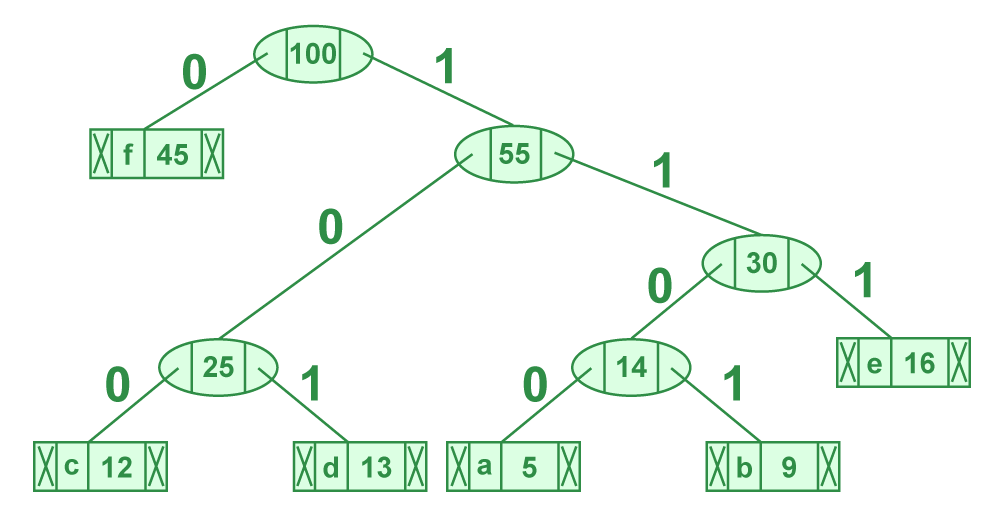
\includegraphics[width=\linewidth]{png/huffman.png}
    \caption{Exemple d'un arbre de Huffman.}
    \label{fig:enter-label}
\end{figure}
Tot aquest procés construeix la nostra classe de Huffman. Aquesta classe encapsula les funcionalitats necessàries per generar i utilitzar l'arbre de Huffman en la compressió i descompressió de dades.

\subsection{Gestió de concurrència} 
Com es costum en les nostres pràctiques, la interfície s'executa en el seu propi thread, a més, cada execució d'un \texttt{Runnable} es fa sobre un thread dins un \texttt{ExecutorService}.
A més, es controla l'aturada controlada dins els processos amb la funció aturar() de \texttt{Comunicar}.

Dins cada procés, també s'utilitza la concurrència per guanyar rendiment:
\begin{itemize}
    \item A l'hora de crear claus, si varis nombres primers no depenen entre sí es pot calcular paral·lelament
    \item A l'hora de tractar amb fitxers, es divideix el fitxer en parts per a cada nucli per a poder operar més rapid
\end{itemize}

\subsection{Visualització i interacció amb l'usuari}
La finestra principal ofereix les següents funcionalitats: permet encriptar o desencriptar un arxiu, gestionar les claus emmagatzemades i controlar els diferents processos en execució.


\begin{figure}[H]
    \centering
    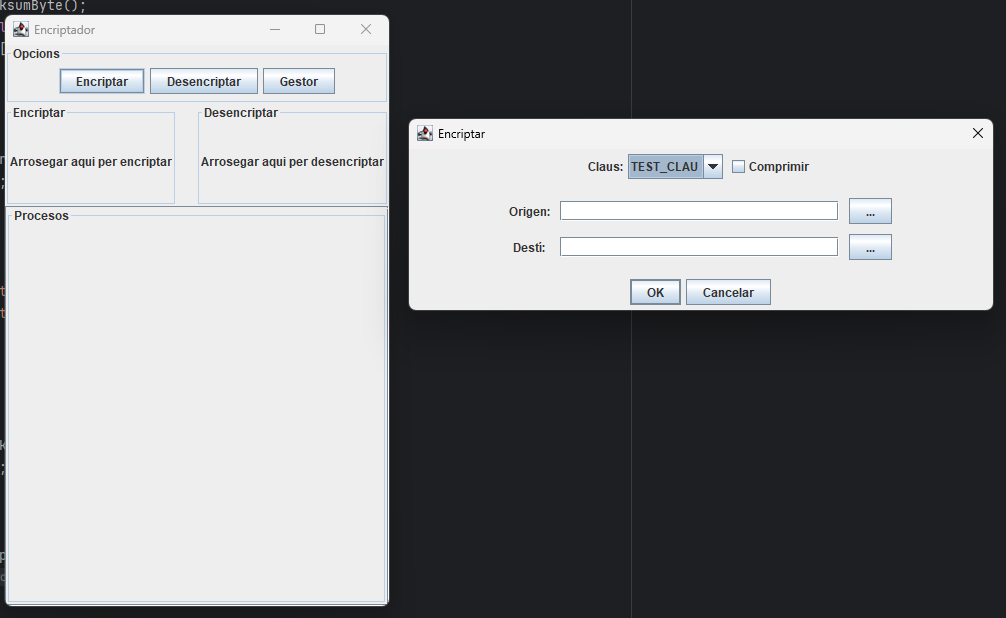
\includegraphics[width=0.45\textwidth]{png/finestra.png}
    \caption{Finestra principal amb modal d'encriptació}
    \label{fig:enter-label}
\end{figure}
A més, durant l'execució del programa s'utilitzen finestres modals per mostrar informació addicional o per demanar a l'usuari l'entrada d'informació

\begin{figure}[H]
    \centering
    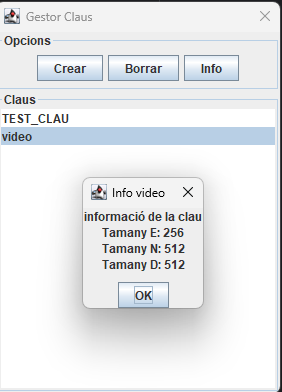
\includegraphics[width=0.5\linewidth]{png/modal.png}
    \caption{Modal del Gestor de Claus amb informació sobre una clau}
    \label{fig:enter-label}
\end{figure}

\subsection{Flux de control i comunicació}

El flux de control i la comunicació entre components segueixen fidelment el patró Model–Vista–Controlador (MVC). La classe \texttt{Main} actua com a controlador principal, gestionant els esdeveniments de la interfície gràfica i delegant les operacions al model de manera asincrònica. Per tal de garantir una arquitectura desacoblada i modular, s'ha dissenyat una interfície pròpia anomenada \texttt{Comunicar}, que defineix un conjunt de mètodes estàndard per a la comunicació entre la vista, el controlador i els processos del model.

\paragraph{Interfície \texttt{Comunicar}}

Aquesta interfície inclou operacions com ara:

\begin{itemize}
  \item \texttt{crearClau()}: Sol·licita la creació d'una nova clau.
  \item \texttt{encriptar()} i \texttt{desencriptar()}: activen els processos corresponents.
  \item \texttt{comunicar(String msg)}: canal de comunicació genèric per enviar missatges i estats entre components.
  \item \texttt{actualitzar()}: utilitzat per actualitzar la vista quan hi ha canvis en les dades.
  \item \texttt{aturar()}: Sol·licita la aturada d'un procés en execució.

\end{itemize}

Aquesta interfície és implementada pel controlador \texttt{Main}, i és passada als components que en necessiten accés, com ara la classe \texttt{Finestra} i \texttt{EncriptadorDesencriptador}.

\paragraph{Controlador i gestió de tasques}

Per garantir una execució fluida i no bloquejant, el controlador empra un \texttt{ExecutorService} amb 3 fils d'execució:

\begin{lstlisting}[language=Java]
private ThreadPoolExecutor executor = (ThreadPoolExecutor) Executors.newFixedThreadPool(3);
\end{lstlisting}

Això permet executar varis procesos de forma concurrent, sense sobrecarregar el sistema.
La crida a, per exemple, encriptar es fa així:

\begin{lstlisting}[language=Java]
@Override
public void encriptar(int id, String kName, String filePath, String outPath, boolean comprimir) {
    EncriptadorDesencriptador ed = new EncriptadorDesencriptador(id, kName);
    executar(id, ed, () -> {ed.encriptar(id, filePath, outPath, comprimir);});
}
\end{lstlisting}

Tant \texttt{RSA} i \texttt{EncriptadorDesencriptador}) implementa la interfície \texttt{Runnable} i \texttt{Comunicar}, un cop finalitzat el seu procés, pot comunicar-se amb el controlador a través del mètode \texttt{finalitzar()}.

\paragraph{Patró \emph{Singleton} i compartició de dades}

La classe \texttt{Main} s’implementa com un \emph{singleton}, de manera que
l’únic punt d’accés global al controlador és el mètode
\texttt{getInstance()}.  
Això permet:

\begin{enumerate}
  \item Compartir el mateix objecte \texttt{Dades} entre tots els components:
        el model és creat una sola vegada dins \texttt{Main} i recuperat des
        de qualsevol lloc amb:
\begin{lstlisting}[language=Java]
Dades dades = Main.getInstance().getDades();
\end{lstlisting}

  \item Facilitar les crides de la vista cap al controlador sense afegir
        dependències dures. 

  \item Garantir coherència de l’estat: com que tots els processos i la
        vista treballen sobre la mateixa instància de \texttt{Dades}, no hi ha
        duplicació d’informació.  A més, qualsevol modificació es fa sempre
        dins el fil gestionat per l’\texttt{ExecutorService}; la vista només
        llegeix els resultats mitjançant \texttt{SwingUtilities.invokeLater},
        evitant condicions de carrera.
\end{enumerate}

D’aquesta manera, el \emph{singleton} no trenca la separació de capes sinó que
serveix com a mecanisme de registre centralitzat perquè tots els actors
 comparteixin l’estat i es comuniquin mitjançant la
interfície \texttt{Comunicar}.


\paragraph{Desacoblament i comunicació estructurada}

Aquest enfocament modular permet que el model i la vista no es coneguin directament entre ells. El model, encapsulat en classes com \texttt{EncriptadorDesencriptador} i \texttt{Dades}, pot operar de manera independent i només comunica resultats a través del controlador. \newline
La vista, representada per la classe \texttt{Finestra}, també opera exclusivament mitjançant la interfície \texttt{Comunicar}, invocant mètodes sense dependre de la implementació específica del model.\newline

Aquesta arquitectura ofereix una gran flexibilitat i facilita la integració de nous mètodes d'encriptació (com el AES), ja que aquests només necessiten accedir a les dades i notificar el controlador de l'estat de l'execució. Alhora, permet una gestió eficaç d'errors i estats mitjançant missatges textuals controlats centralment al \texttt{Main}.


\subsection{Decisions de disseny i extres implementats}
Per tenir centralitzat les diferents funcionalitats, s'ha obtat per tenir poques classes, però especialitzades en el seu àmbit, per exemple: \texttt{RSA} s'encarrega de tot el relacionat amb les claus RSA, des de generarles, guardar-les en arxius, llegir-les, etc. El mateix passa amb \texttt{EncriptadorDesencriptador}, que conté tota la funcionalitat per encriptar i desencriptar un arxiu, encara que utilitza les classes \texttt{RSA} i \texttt{CryptHeader} com a suport.

Per a l'extra de comprimir, s'ha agafat el model de la pràctica 4, aquest model ha estat modificat per ser més compatible, però gràcies al MVC han estat canvis menors.
Per a l'extra de mostrar el temps s'ha reutilitzat, sense pràcticament haver fet cap canvi, les barres de càrrega de la pràctica 5.

La classe \texttt{PrimoProbable} és la publicada a l'aula digital, ja que no és necessari reinventar la roda, a més, \texttt{RSA} està basat també en el projecte de classe, però modificat substancialment per aprofitar la concurrència i la gestió de claus. 

\section{Resultats i Comparació} 
En aquesta secció es posa a prova el funcionament del xifrat. Amb l'obtenció del temps d'execució de diferents claus es pot fer una comparativa del rendiment segons el tamany d'aquesta.




\begin{table}[H]
\centering
\caption{Classificació del temps de generació d'una clau segons el seu tamany}
\label{tab:xarxa}
\begin{tabular}{|c|c|}
\hline
\textbf{N} & \textbf{segons}  \\
\hline
64  & 0,011   \\
128  & 0,610   \\
256 & 0,467      \\
512 & 0,687   \\
1024 & 19,256       \\
\hline
\end{tabular}
\end{table}

\begin{table}[H]
\centering
\caption{Classificació del temps (s) d'encriptació i desencriptació segons el tamany de la clau}
\label{tab:clasificacion}
\begin{tabular}{|c|c|c|c|c|}
\hline
\textbf{N} & \textbf{encriptar no c} & \textbf{desencriptar no c} & \textbf{encriptar c} & {desenciptar c} \\
\hline
64   & 1.699 & 0,603 & 0,919 & 0,838 \\
128  & 2.152 & 3,304 & 2,577 & 3,782 \\
256  & 11,175 & 21,109 & 12,863 & 21,605 \\
512  & 76,532 & 147,109 & 80,045 & 149,684 \\
\hline
\end{tabular}
\end{table}

\begin{table}[H]
\centering
\caption{Diferencia de pes comprimit i sense}
\label{tab:clasificacion}
\begin{tabular}{|c|c|c|}
\hline
\textbf{N} & \textbf{no comprimit (MB)} & \textbf{comprimit (MB)} \\
\hline
128  & 11,0 & 9,98 \\
256  & 21,9 & 19.9 \\
\hline
\end{tabular}
\end{table}

Els resultats obtinguts es poden representar de manera visual mitjançant un gràfic de barres, que permet comparar fàcilment el rendiment dels diferents classificadors.

Els resultats permeten observar una clar augment del temps, de forma no lineal, d'execució en la mesura que augmenta N, també es pot intuir que el temps de desencriptació suposa el doble de temps respecte l'encriptació.

També una altre conclusió que es pot treure dels resultats es que el fet de comprimir o no l'arxiu encriptat afecti significativament al rendiment general.

Finalment, encara que els arxius siguin molt més grans xifrats que els originals, comprimir l'arxiu redueix un 10\% del tamay original.

\section{Conclusions} 
En conclusió, aquesta pràctica ha estat molt interessant per a mi, la criptologia es una branca que es dona de reüll a les diferents assignatures de les que he estat estudiant, i poder treballar amb ella, encara que sigui a un nivell bàsic, ha estat enriquidor.
Tenint el compte la limitant de haver de compaginar aquesta pràctica amb exàmens i altres treballs puc dir que estic orgullós, encara que amb més temps hagués pogut fer altres coses, com implementar claus híbrides amb AES, i optimitzar, encara més, la encriptació, especialment a nivell espacial.
També ha estat una ajuda poder reutilitzar diferents components d'altres pràctiques, sense això segurament hagués necessitat un altre dia de feina.


\bibliographystyle{IEEEtran}
\begin{thebibliography}{1}

\bibitem{RSA} RL. Rivest, A. Shamir, L. Adleman, \emph{A Method for Obtaining Digital
Signatures and Public-Key Cryptosystems} \url{https://people.csail.mit.edu/rivest/Rsapaper.pdf}

\bibitem{hammersley1964} J.~M. Hammersley i D.~C. Handscomb, \emph{Monte-Carlo-Methods}, Chapman \& Hall, 1964.

\bibitem{pubkey} Martin E. Hellman \emph{An Overview of Public Key Cryptography} \url{https://www-ee.stanford.edu/~hellman/publications/31.pdf}

\bibitem{huffman1952} D.~A. Huffman.
\newblock A method for the construction of minimum‐redundancy codes.
\newblock \emph{Proceedings of the IRE}, 40(9):1098–1101, 1952.

\bibitem{gamma1994} E.~Gamma, R.~Helm, R.~Johnson i J.~Vlissides, \emph{Design Patterns: Elements of Reusable Object-Oriented Software}, Addison-Wesley, 1994.

\bibitem{miller} Keith Conrad \emph{THE MILLER–RABIN TEST} \url{https://kconrad.math.uconn.edu/blurbs/ugradnumthy/millerrabin.pdf}


\bibitem{gafter1999} J.~Gafter, “Swing Architecture and Concepts,” JavaOne Conference, 1999.
\end{thebibliography}



\end{document}


